\documentclass[12pt]{article}
\usepackage{xcolor}

\usepackage[margin=1in]{geometry}
\usepackage{amssymb}
\usepackage{amsmath}
\usepackage{bm}
\usepackage{xcolor}

\usepackage[english]{babel}
\usepackage[utf8]{inputenc}
\usepackage{algorithm}
% \usepackage{algpseudocode}
% \usepackage{algorithmic}
\usepackage[noend]{algpseudocode}
\usepackage{enumitem}


\def\R{\rm I\!R}
\def\x{\bm{x}}
\DeclareMathOperator*{\argmax}{arg\,max}
\DeclareMathOperator*{\argmin}{arg\,min}

\renewcommand{\algorithmicrequire}{\textbf{Input:}}
\renewcommand{\algorithmicensure}{\textbf{Output:}}
\graphicspath{{Figures/Experiment_results/SGD/}{./}} 
\captionsetup[figure]{font=scriptsize,labelfont=bf}


\title{SGD Quantile Estimation Experiment}
\date{\vspace{-5ex}}

\begin{document}
\maketitle

\section{Introduction}

% \subsection{Aims}
This experiment has two purposes. The first is to show quantile estimation with SGD works \textcolor{blue}{ under some circimstances (?)}.
The second aim is to investigate how different settings of the problem effect the estimation performance. Specifically, we are interested in the following aspects: data distribution, data size, data ordering, quantile value and sgd step size.
In the experiment, multiple ordered datasets are generated as input data streams, based on which the calculated and estimated quantile values are computed. Results of both quantiles are compared after processing. We want to compare the performance of quantile estimation over different settings.
\\\\
\textcolor{blue}{
\textbf{I think this is another experiment?}
\\    
This experiment also aims at the comparison between Frugal algorithm and SGD algorithm, by which we want to show that those two algorithms are ``equivalent". 
\\
(Does it mean SGD estimation works?)}
% To test the SGD quantile estimation as a valid alternative for quantile estimation, this experiment computes both estimated and calculated values for quantiles, and evaluates whether the difference between the results is acceptable.
% \\\\
% Do I explain the second goal...?


\section{Methodology}
The process by which we experiment on SGD quantile estimation can be briefly outlined as follows:
\begin{enumerate}
    \item Generate an SGD quantile estimate of benchmarking setting.
    \item For each setting category, generate the other quantile estimate with accordingly changed settings.
    \item Compare the performances of both groups of estimate value.
\end{enumerate}
For step 2, the detailed generation steps for a quantile estimate are:
\begin{enumerate}[label=(\roman*)]
    \item Select a set of data streams (ordered datasets) derived from some statistical distributions.
    \item For each $\tau$-quantile, determine a ground truth value from the distribution and calculate a empirical value from the data stream.
    \item For each $\tau$-quantile, calculate the SGD estimate value from the data stream, record both the process and the result of estimation.
    % \item \textcolor{blue}{
    %     Compare Frugal algorithm and SGD algorithm on data streams of the same setting.
    % }
    \item Compute normalized error value for quantile estimates as a measurement of similarity between empirical and estimate value. The error value is computed from both values.
\end{enumerate}

\subsection{Benchmarking Estimate Setting}
The benchmarking setting of the SGD quantile estimate is:
    \begin{enumerate}
        \item Data stream:
            \begin{itemize}
                \item Distribution: Gaussian distribution: mean = 2, standard deviation = 18
                \item Data size: 1000 i.i.d. (independent and individual distributed) random samples
                \item Multiple generations: true. 10 data streams of the same setting are generated
                \item Multiple shuffles: false. No data streams are generated as a shuffled version of another
            \end{itemize}
        \item Step size: constant value 1
    \end{enumerate}
\textcolor{blue}{
Reason to choose it as a benchmark: not quite sure about this
\\    
distribution: easy to compare with different "shaped" distribution (e.g. gau 2), 
\\
multiple generations: to compare with the same generation but different sequence of data stream. 
\\
step size: the most trivial one, derived from Frugal method}
\\
A detailed description of the benchmarking estimate generation is shown in the subsection 2.2.

\subsection{SGD Quantile Estimate Generation}
To ensure the consistency of quantile estimate construction, the generation methods for a specific setting are restricted.
In this section, we will introduce the rules and steps for generation in details.

\subsubsection{Data Stream Set Generation}
A total of 4 distributions are used in this experiment.
Eah data stream is a set of 1 dimensional data points randomly sampled from one of the distributions. In order to show how the amount of data points might affect the performance, there are 3 different settings for the data size $N$. 
\\\\
Each data stream set is composed of a number of data streams. For a statistically more accurate results on the experiment, a group of data streams of the same settings are generated. When investigating the impact of data sequence has on quantile estimation, one data stream will be shuffled to for the generation to differently ordered data steams. To sum up, a data stream set is either a combination of data streams generated from same distribution and data size setting, or the permutations of one same data stream. We generate the data stream set under this settings:

\begin{itemize}
    \item Distribution: 4 statistical distributions. The 4 distributions are:
        \begin{itemize}
            \item Gaussian distribution 1: mean = 2, standard deviation = 18
            \item Gaussian distribution 2: mean = 0, standard deviation = 0.001
            \item Exponential distribution: rate = 1
            \item Mixed Gaussian distribution: a mix of five different gaussian distributions
        \end{itemize}
    \item Data size: 100, 1000, 100000
    \item Multiple generations: True or false. Generate 10 data streams for the set if true.
    \item Multiple shuffles:  True or false. Shuffle the data stream 10 times for the set if true.
\end{itemize}


\subsubsection{True and Empirical Quantile Calculation}
The true quantile values are the quantile values for the distributions which the data streams are derived from. They are calculated by the maths functions for quantile computation. All except the mixed gaussian distribution has a relatively easy function for quantile calculation. For the mixed distribution, the empirical quantile value from a large amount of sampling is taken for the true value. By this means, the empirical value is expected to be close enough to the true quantile value such that the evaluation of results is not much affected \textcolor{blue}{(needs more justification?)}. In this experiment, a total of 100,000,000 samples are generated for the calculation. For a certain $\tau$, there is only one true quantile value for one distribution.
\\\\
The empirical quantile value is the quantile value calculated from the data steam instead of the distribution. For a certain $\tau$, no matter what the ordering is, there is only one empirical quantile value for one data stream, but there can be multiple quantile values for one distribution.

\subsubsection{SGD Quantile Estimation}

The parameter of SGD quantile estimation is important. The current settings for step size $\alpha_k$ are:
\begin{itemize}
    \item Constant number: $\alpha_k =1$
    \item Decrease when k increases: $\alpha_k = \frac{2}{\sqrt{k}}$
    \item Decrease when k increases (smaller size): $\alpha_k = \frac{0.002}{\sqrt{k}}$
\end{itemize}
where $k$ is the index of step count.

% \section{Frugal and SGD algorithm}

% Frugal algorithm is proposed for quantile estimation as well. In this experiment, we want to compare the two algorithms and show they have similar performance for same data streams. In this experiment, data streams are generated from all 4 distributions, and the step size for SGD quantile estimation is set to constant 1.

\subsubsection{Error Computation}

An error measurement is proposed in order to evaluate the performance of quantile estimation. The error value represents the difference between empirical and estimated quantile value. For one data stream, the error function for its $\tau$-quantile is first defined as $E^{(\tau)} = | q_{batch}^{(\tau)} - q_{sgd}^{(\tau)} |$, where $E^{(\tau)}$ stands for the error, $q_{batch}^{(\tau)}$ for empirical quantile value and $q_{sgd}^{(\tau)}$ for SGD estimate value. For a specific data stream, a smaller $E^{(\tau)}$ means the estimation for the $\tau$-quantile has a better accuracy. Generally, for $n$ data streams of same size and distribution, we take the mean of the error value $\overline{E^{(\tau)}}$, where 
    $$
        \overline{E^{(\tau)}} = \frac{1}{n}\sum_{i=1}^{n} E^{(\tau)}_{i}
    $$
where $E^{(\tau)}_{i}$ is the error value of $\tau$-quantile for the $i$th data stream. To compare the performance of different settings of SGD estimation, we can now compare the $\overline{E^{(\tau)}}$ value for each setting.
\\\\
 Despite the capability of accuracy comparison, there is still room for improvement for this preliminary error measurement. 
% distribution
 First, the limitation of data distribution. The comparison is only available for data streams generated from the same distribution, since a different distribution has difference density of data points for the same $\tau$ value, leading to a failure of error comparison. For example, a data stream generated from uniform distribution $\mathcal{U}(0,1)$, the error value $\overline{E^{(0.1)}} = 2$ is a bad estimation, because 2 is even greater than the difference between the minimal and maximal value of the distribution ($2 > |0-1|$). However, for a data stream sampled from uniform distribution $\mathcal{U}(0,10^{10})$, $\overline{E^{(0.1)}} = 2$ might be a really accurate result, given how low the density is around its 0.1-quantile. 
% tau
 Second, the limitation of $\tau$ value. Similarly with the distribution problem, different $\tau$ values in the same distribution may have varied density. For example, for a gaussian distribution, $\overline{E^{(0.01)}} = \overline{E^{(0.5)}}$ means that the estimation is better for 0.01-quantile than 0.5-quantile, since the distribution is denser around the middle than its outlier.
% how it works
 Third and more importantly, it is incapable of showing if the estimation "works". Specifically, for some number $x$, we cannot find a reasonable explanation for the statement ``the estimate is accurate enough because we have $\overline{E^{(\tau)}} \leq x$''. Since for any $x$, we could find an example from the first two issues as a counter example. To solve those problems, a more general comparison of accuracy should be enabled by the new error measurement.
\\\\
In the new version of error value calculation, true quantile value of a data distribution $q_{true}^{(\tau)}$ is involved, so that $E^{(\tau)}$ is normalized by $|q_{batch}^{(\tau)} - q_{true}^{(\tau)}|$. It is now defined as
$$
    E^{(\tau)} = \frac{|q_{batch}^{(\tau)} - q_{sgd}^{(\tau)}|}
                      {|q_{batch}^{(\tau)} - q_{true}^{(\tau)}|}
$$
So that the accuracy of $q_{sgd}^{(\tau)}$ is compared with the accuracy of $q_{batch}^{(\tau)}$. The above problem is solved because 
\textcolor{blue}{(I am not sure about this part)\\
    $
    q_{batch} - q_{true}
    $
    is the normalizer which reduces the effect of unevenly distributed density among different distributions and different quantile values.
}

\subsection{Performance Comparison}
Plots that shows the performance of quantile estimate results, processes and its error values.

Result plot: shows the estimate results of $q_{batch}$ and $q_{sgd}$. The clustering of both values are obvious

Process plot: shows the processes.

Error plot: shows the normalized error value for every data stream of this setting.

All of them show the summarized visualization of multiple generation of estimate values.


\pagebreak
\section{Observations}

\subsection{Distribution}
Except for default setting of gaussian 1 distribution, two other distributions are included: the mix gaussian distribution and the exponential distribution.

\subsubsection{Estimate results on different distributions}
\begin{figure}[H] % [h] forces the figure to be output where it is defined in the code (it suppresses floating)
	\centering
    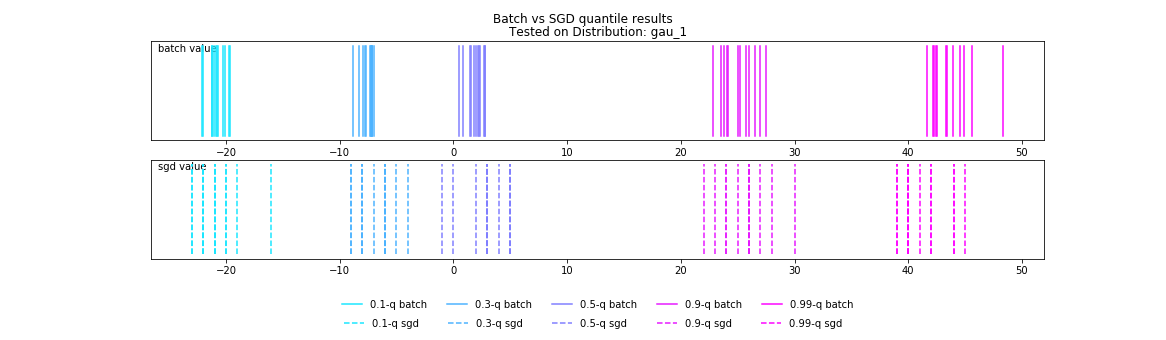
\includegraphics
    [width=1\columnwidth]
    {distro/gau_1_res.png} % Example image
	\caption{
		SGD Estimate Results from Gaussian 1 Distribution
	}
\end{figure}

\begin{figure}[H] % [h] forces the figure to be output where it is defined in the code (it suppresses floating)
	\centering
    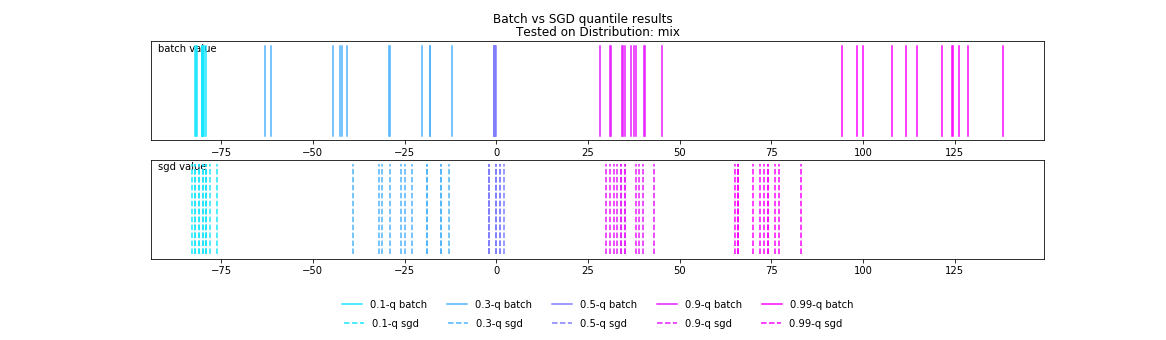
\includegraphics
    [width=1\columnwidth]
    {distro/mix_res.png} % Example image
	\caption{
		SGD Estimate Results from Mix Distribution
	}
\end{figure}

\begin{figure}[H] % [h] forces the figure to be output where it is defined in the code (it suppresses floating)
	\centering
    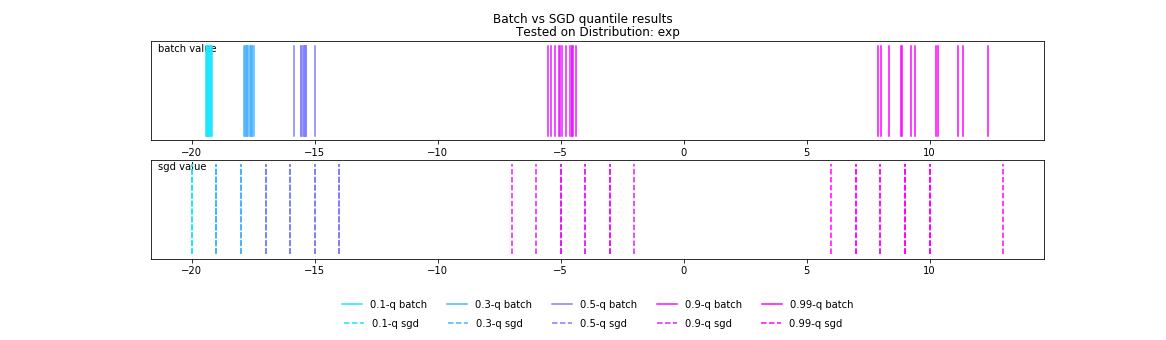
\includegraphics
    [width=1\columnwidth]
    {distro/exp_res.png} % Example image
	\caption{
		SGD Estimate Results from Exponential Distribution
	}
\end{figure}



\subsubsection{Estimate processes on different distributions}
\begin{figure}[H] % [h] forces the figure to be output where it is defined in the code (it suppresses floating)
	\centering
    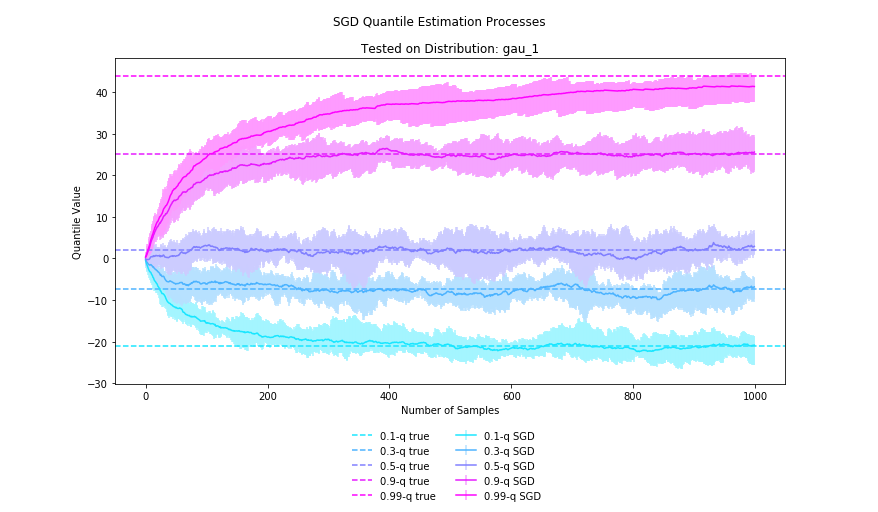
\includegraphics
    [width=1\columnwidth]
    {distro/gau_1_proc.png} % Example image
	\caption{
		SGD Estimate Process from Gaussian 1 Distribution
	}
\end{figure}

\begin{figure}[H] % [h] forces the figure to be output where it is defined in the code (it suppresses floating)
	\centering
    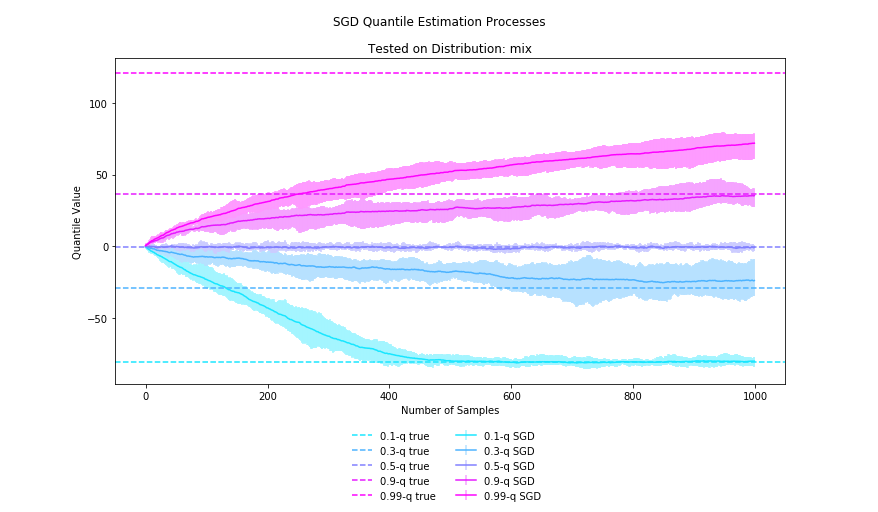
\includegraphics
    [width=1\columnwidth]
    {distro/mix_proc.png} % Example image
	\caption{
		SGD Estimate Process from Mix Distribution
	}
\end{figure}

\begin{figure}[H] % [h] forces the figure to be output where it is defined in the code (it suppresses floating)
	\centering
    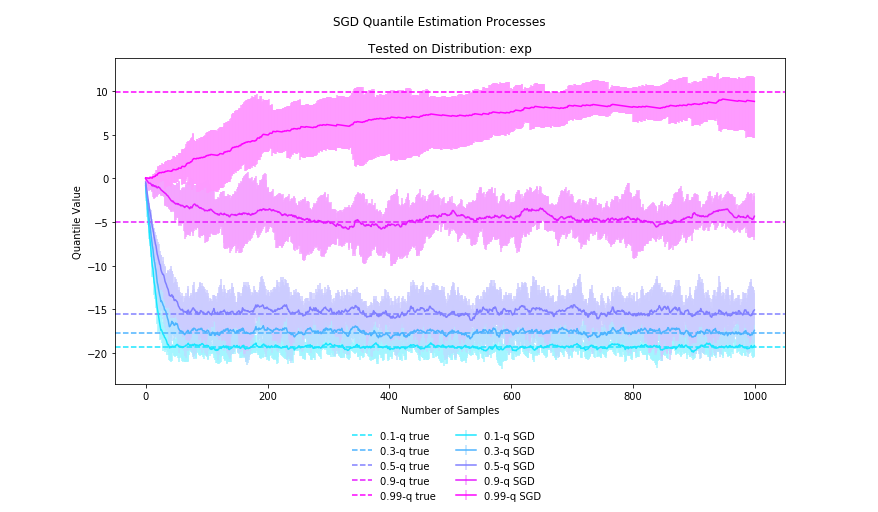
\includegraphics
    [width=1\columnwidth]
    {distro/exp_proc.png} % Example image
	\caption{
		SGD Estimate Process from Exponential Distribution
	}
\end{figure}

\subsubsection{Estimate Error Value on different distributions}
\begin{figure}[H] % [h] forces the figure to be output where it is defined in the code (it suppresses floating)
	\centering
    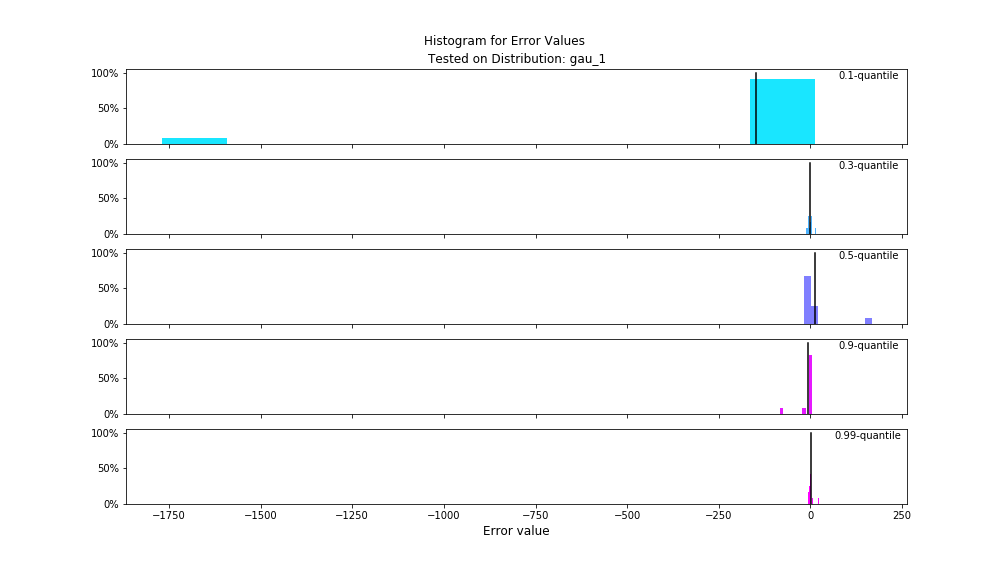
\includegraphics
    [width=1\columnwidth]
    {distro/gau_1_err.png} % Example image
	\caption{
		SGD Estimate Error from Gaussian 1 Distribution
	}
\end{figure}

\begin{figure}[H] % [h] forces the figure to be output where it is defined in the code (it suppresses floating)
	\centering
    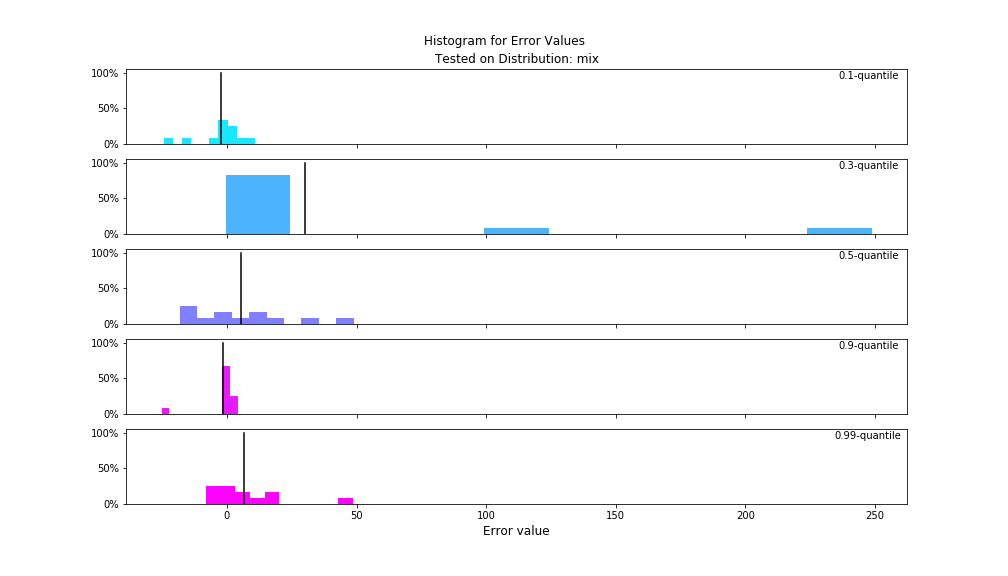
\includegraphics
    [width=1\columnwidth]
    {distro/mix_err.png} % Example image
	\caption{
		SGD Estimate Error from Mix Distribution
	}
\end{figure}

\begin{figure}[H] % [h] forces the figure to be output where it is defined in the code (it suppresses floating)
	\centering
    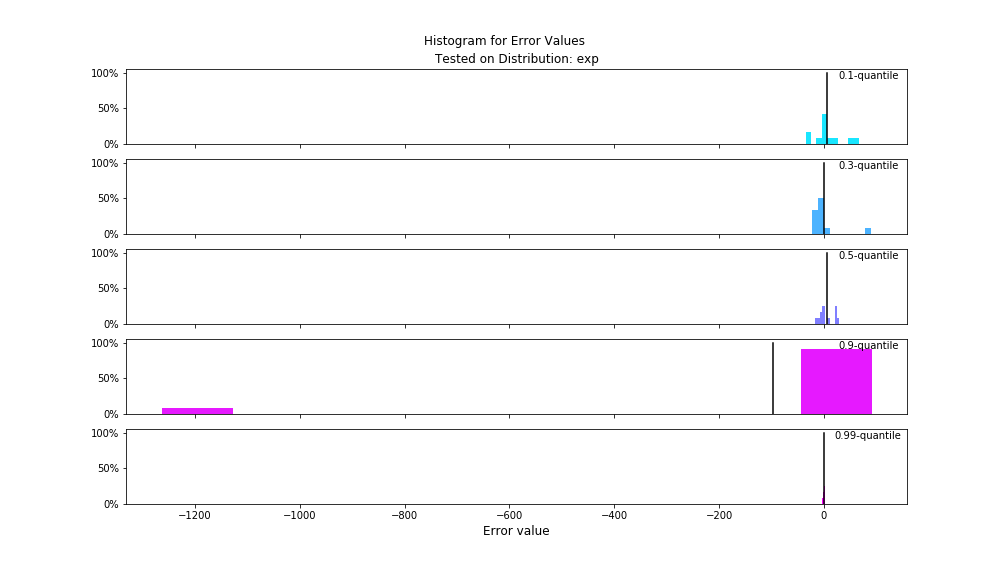
\includegraphics
    [width=1\columnwidth]
    {distro/exp_err.png} % Example image
	\caption{
		SGD Estimate Error from Exponential Distribution
	}
\end{figure}

\pagebreak
\subsection{Data Size}

\subsubsection{Estimate Results on Different Data Size}
\begin{figure}[H] % [h] forces the figure to be output where it is defined in the code (it suppresses floating)
	\centering
    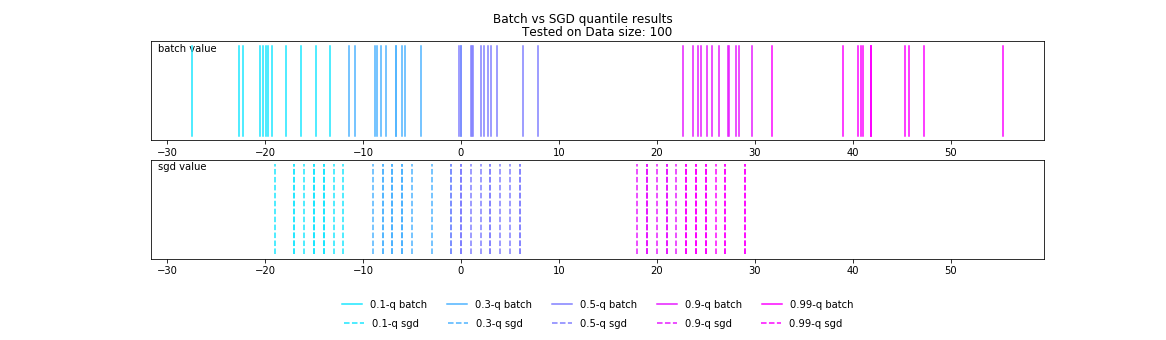
\includegraphics
    [width=1\columnwidth]
    {data_size/100_res.png} % Example image
	\caption{
		SGD Estimate Results from 100 Samples
	}
\end{figure}

\begin{figure}[H] % [h] forces the figure to be output where it is defined in the code (it suppresses floating)
	\centering
    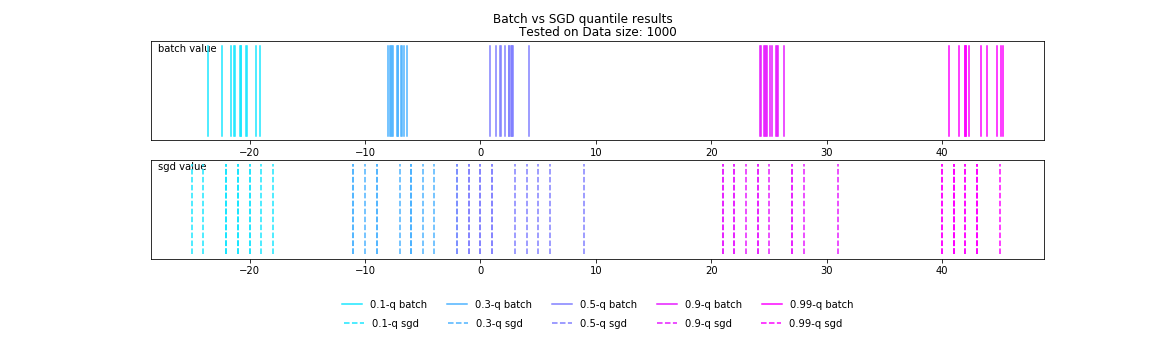
\includegraphics
    [width=1\columnwidth]
    {data_size/1000_res.png} % Example image
	\caption{
		SGD Estimate Results from 1000 Samples
	}
\end{figure}
\begin{figure}[H] % [h] forces the figure to be output where it is defined in the code (it suppresses floating)
	\centering
    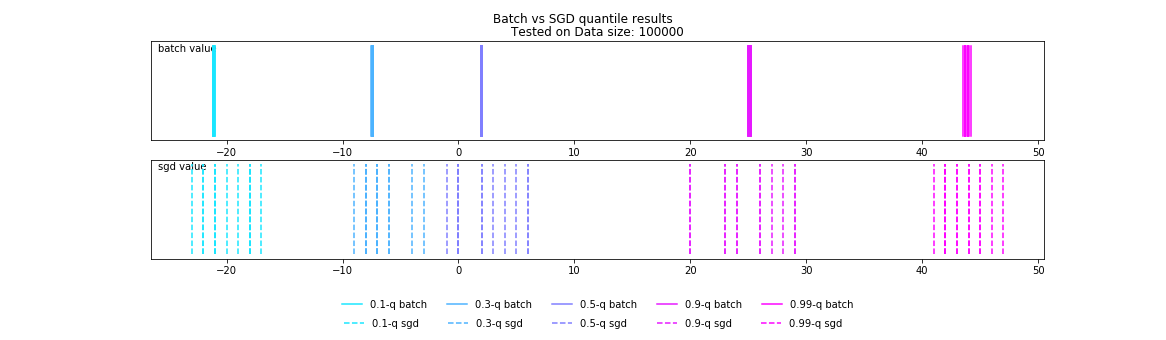
\includegraphics
    [width=1\columnwidth]
    {data_size/100000_res.png} % Example image
	\caption{
		SGD Estimate Results from 100000 Samples
	}
\end{figure}


\subsubsection{Estimate Processes on Different Data Size}

\begin{figure}[H] % [h] forces the figure to be output where it is defined in the code (it suppresses floating)
	\centering
    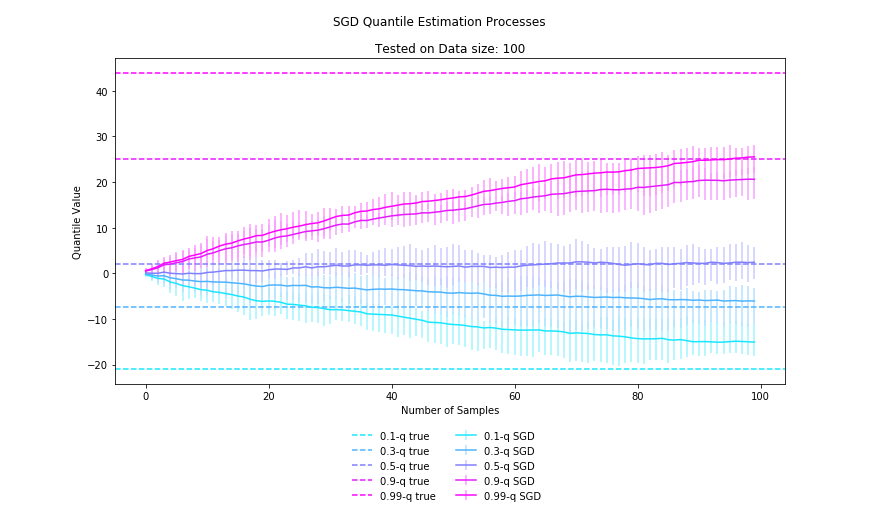
\includegraphics
    [width=1\columnwidth]
    {data_size/100_proc.png} % Example image
	\caption{
		SGD Estimate Process from 100 Samples
	}
\end{figure}

\begin{figure}[H] % [h] forces the figure to be output where it is defined in the code (it suppresses floating)
	\centering
    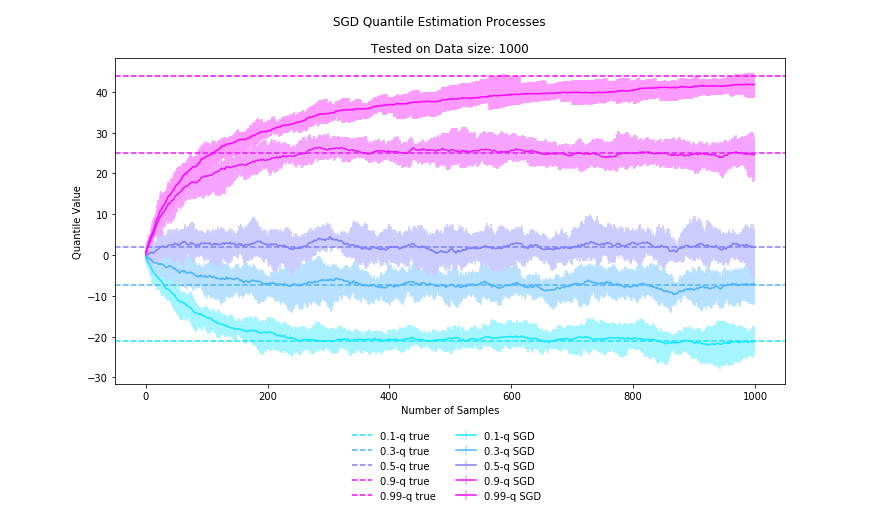
\includegraphics
    [width=1\columnwidth]
    {data_size/1000_proc.png} % Example image
	\caption{
		SGD Estimate Process from 1000 Samples
	}
\end{figure}
\begin{figure}[H] % [h] forces the figure to be output where it is defined in the code (it suppresses floating)
	\centering
    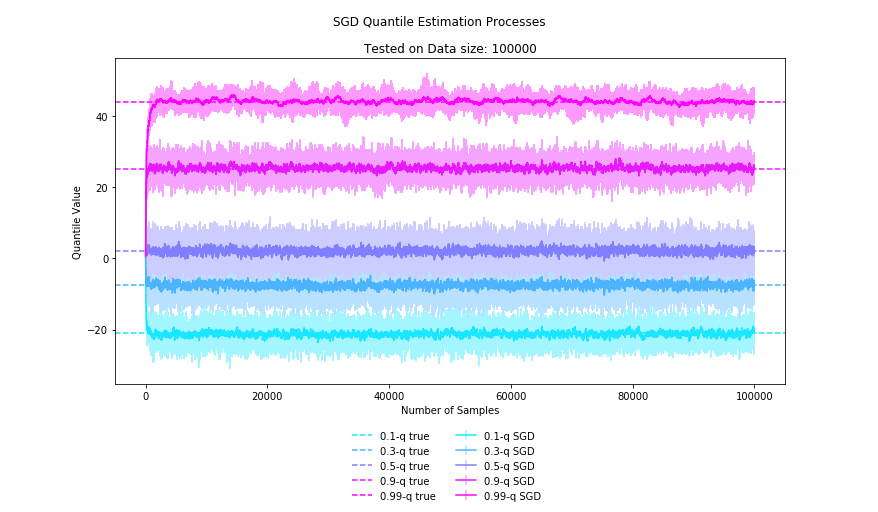
\includegraphics
    [width=1\columnwidth]
    {data_size/100000_proc.png} % Example image
	\caption{
		SGD Estimate Process from 100000 Samples
	}
\end{figure}

\subsubsection{Estimate Error Values on Different Data Size}
\begin{figure}[H] % [h] forces the figure to be output where it is defined in the code (it suppresses floating)
	\centering
    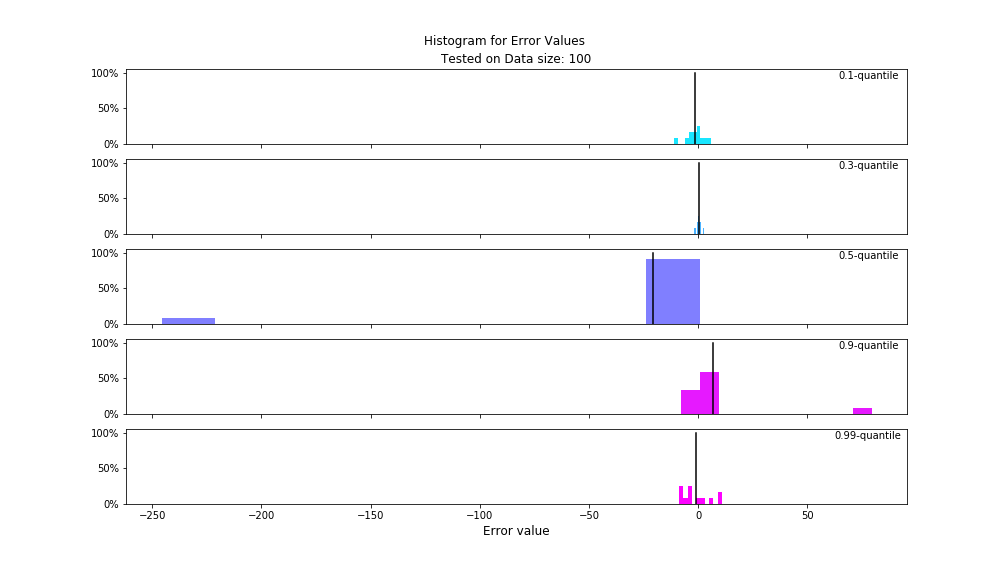
\includegraphics
    [width=1\columnwidth]
    {data_size/100_err.png} % Example image
	\caption{
		SGD Estimate Error from 100 Samples
	}
\end{figure}

\begin{figure}[H] % [h] forces the figure to be output where it is defined in the code (it suppresses floating)
	\centering
    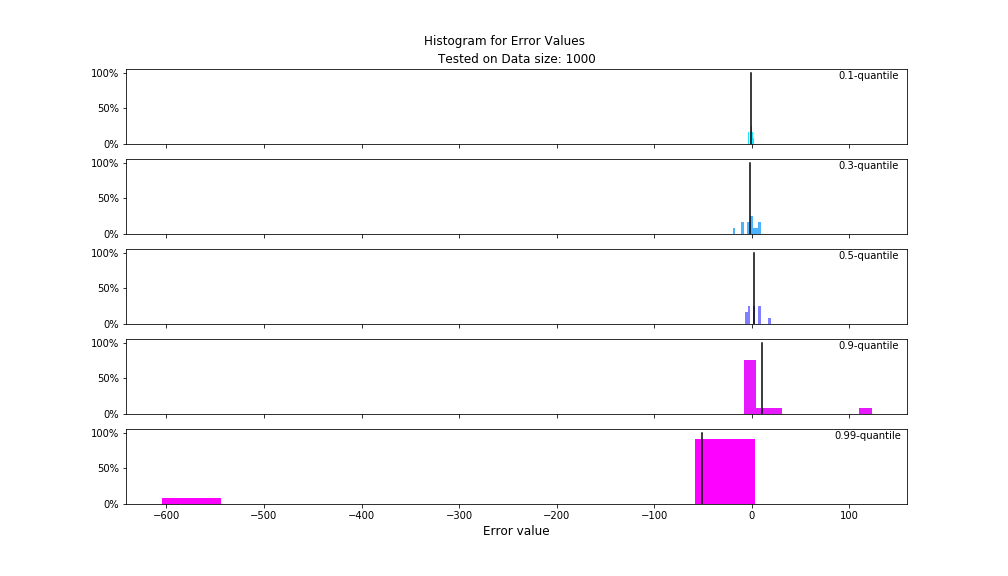
\includegraphics
    [width=1\columnwidth]
    {data_size/1000_err.png} % Example image
	\caption{
		SGD Estimate Error from 1000 Samples
	}
\end{figure}
\begin{figure}[H] % [h] forces the figure to be output where it is defined in the code (it suppresses floating)
	\centering
    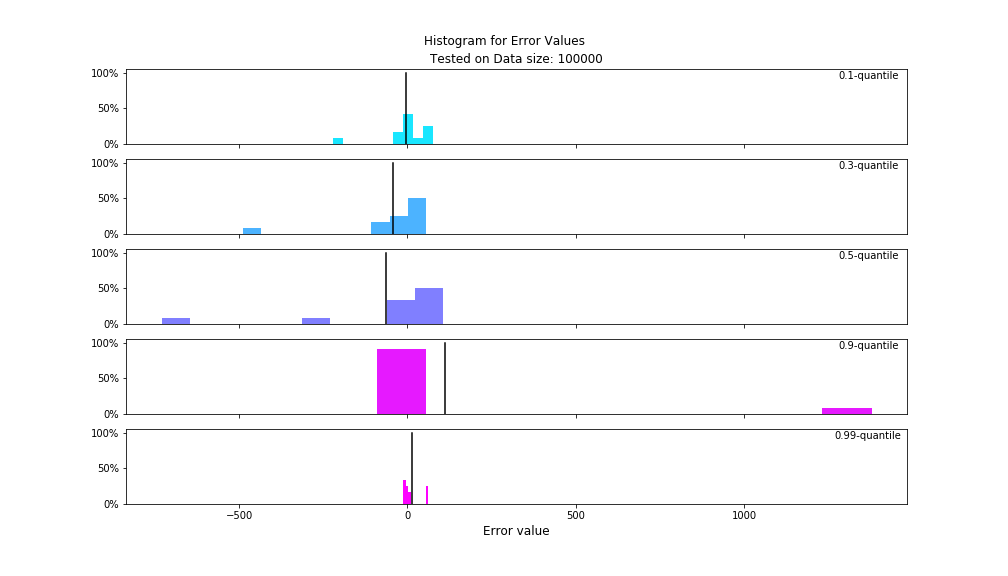
\includegraphics
    [width=1\columnwidth]
    {data_size/100000_err.png} % Example image
	\caption{
		SGD Estimate Error from 100000 Samples
	}
\end{figure}

\pagebreak
\subsection{SGD Step Size}

\subsubsection{Estimate Results on Different SGD Step sizes}
\begin{figure}[H] % [h] forces the figure to be output where it is defined in the code (it suppresses floating)
	\centering
    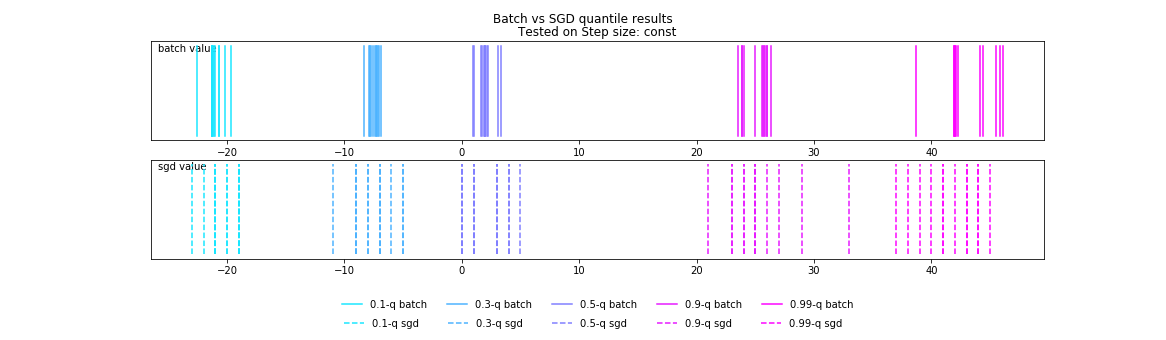
\includegraphics
    [width=1\columnwidth]
    {step_size/const_res.png} % Example image
	\caption{
		SGD Estimate Results from step size $\alpha_k =1 $
	}
\end{figure}

\begin{figure}[H] % [h] forces the figure to be output where it is defined in the code (it suppresses floating)
	\centering
    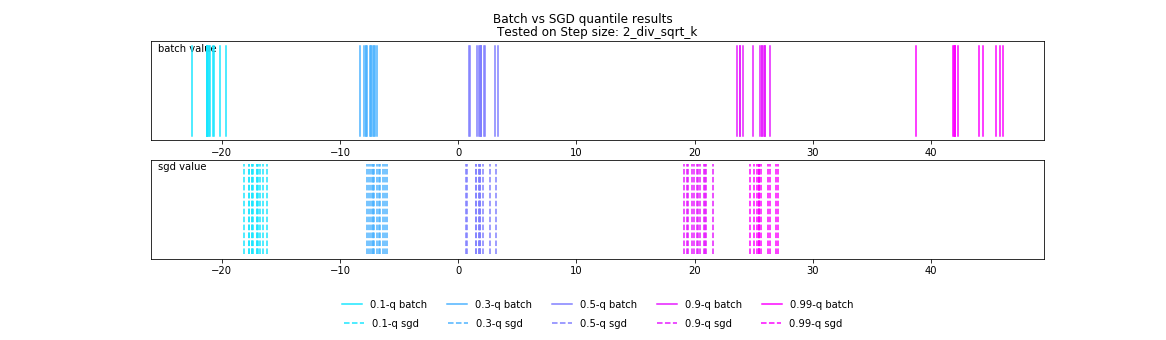
\includegraphics
    [width=1\columnwidth]
    {step_size/2_div_sqrt_k_res.png} % Example image
	\caption{
		SGD Estimate Results from step size $ \alpha_k = \frac{2}{\sqrt{k}}$
	}
\end{figure}

\begin{figure}[H] % [h] forces the figure to be output where it is defined in the code (it suppresses floating)
	\centering
    \includegraphics
    [width=1\columnwidth]
    {step_size/{0.002_div_sqrt_k_res}.png} % Example image
	\caption{
		SGD Estimate Results from step size $ \alpha_k = \frac{0.002}{\sqrt{k}}$
	}
\end{figure}

\subsubsection{Estimate Processes on Different SGD Step sizes}
\begin{figure}[H] % [h] forces the figure to be output where it is defined in the code (it suppresses floating)
	\centering
    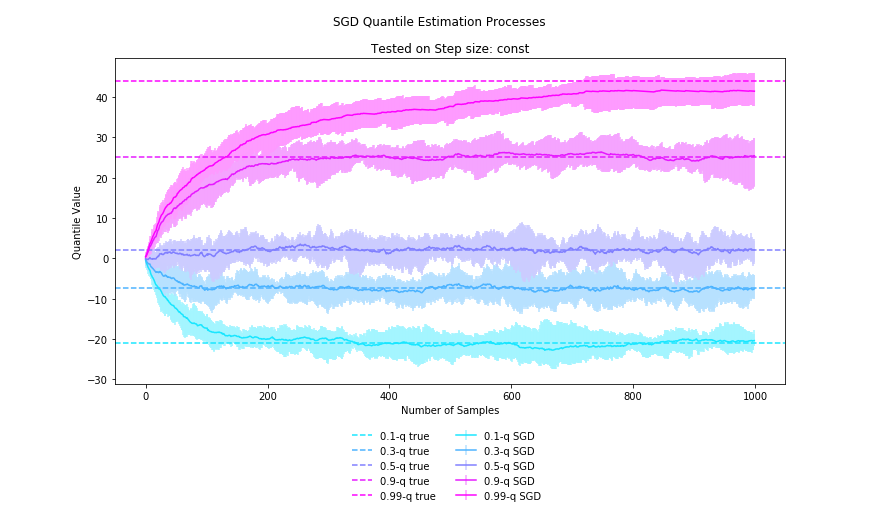
\includegraphics
    [width=1\columnwidth]
    {step_size/const_proc.png} % Example image
	\caption{
		SGD Estimate Process from step size $\alpha_k =1 $
	}
\end{figure}

\begin{figure}[H] % [h] forces the figure to be output where it is defined in the code (it suppresses floating)
	\centering
    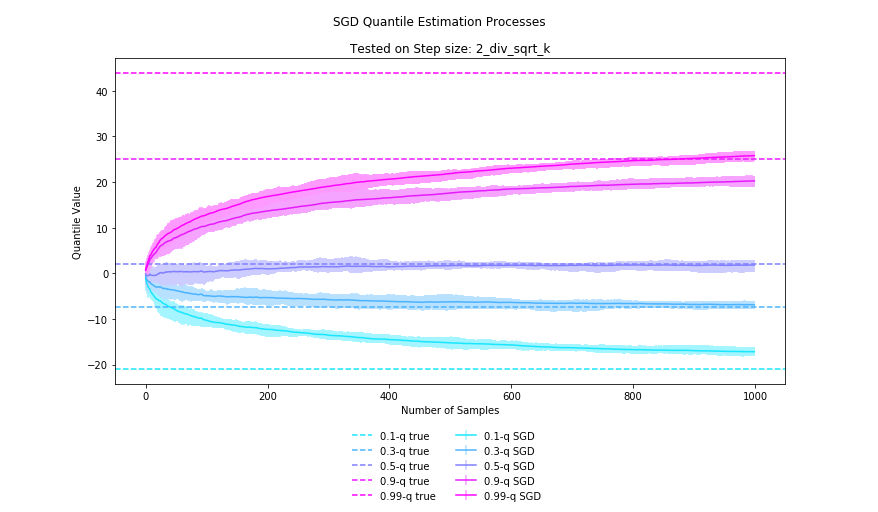
\includegraphics
    [width=1\columnwidth]
    {step_size/2_div_sqrt_k_proc.png} % Example image
	\caption{
		SGD Estimate Process from step size $ \alpha_k = \frac{2}{\sqrt{k}}$
	}
\end{figure}

\begin{figure}[H] % [h] forces the figure to be output where it is defined in the code (it suppresses floating)
	\centering
    \includegraphics
    [width=1\columnwidth]
    {step_size/{0.002_div_sqrt_k_proc}.png} % Example image
	\caption{
		SGD Estimate Process from step size $ \alpha_k = \frac{0.002}{\sqrt{k}}$
	}
\end{figure}

\subsubsection{Estimate Error Values on Different SGD Step sizes}
\begin{figure}[H] % [h] forces the figure to be output where it is defined in the code (it suppresses floating)
	\centering
    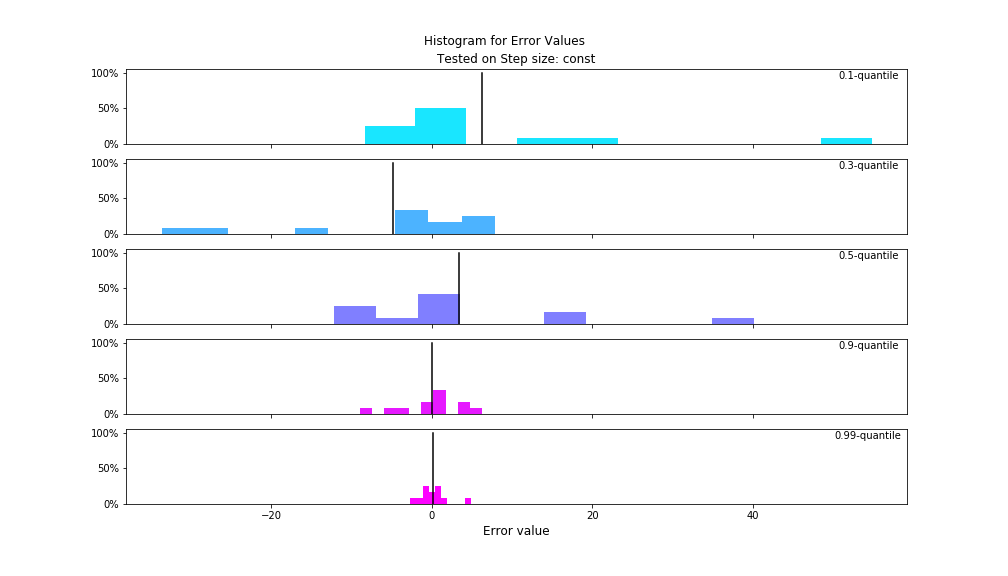
\includegraphics
    [width=1\columnwidth]
    {step_size/const_err.png} % Example image
	\caption{
		SGD Estimate Error from step size $\alpha_k =1 $
	}
\end{figure}

\begin{figure}[H] % [h] forces the figure to be output where it is defined in the code (it suppresses floating)
	\centering
    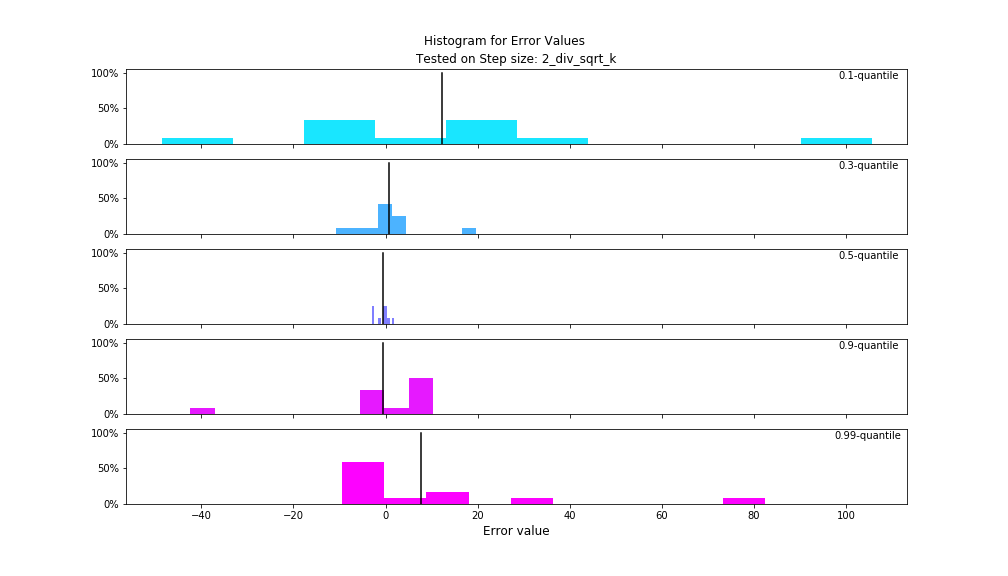
\includegraphics
    [width=1\columnwidth]
    {step_size/2_div_sqrt_k_err.png} % Example image
	\caption{
		SGD Estimate Error from step size $ \alpha_k = \frac{2}{\sqrt{k}}$
	}
\end{figure}

\begin{figure}[H] % [h] forces the figure to be output where it is defined in the code (it suppresses floating)
	\centering
    \includegraphics
    [width=1\columnwidth]
    {step_size/{0.002_div_sqrt_k_err}.png} % Example image
	\caption{
		SGD Estimate Error from step size $ \alpha_k = \frac{0.002}{\sqrt{k}}$
	}
\end{figure}

\pagebreak
\subsection{Ordering of Data Stream}

\begin{figure}[H] % [h] forces the figure to be output where it is defined in the code (it suppresses floating)
	\centering
    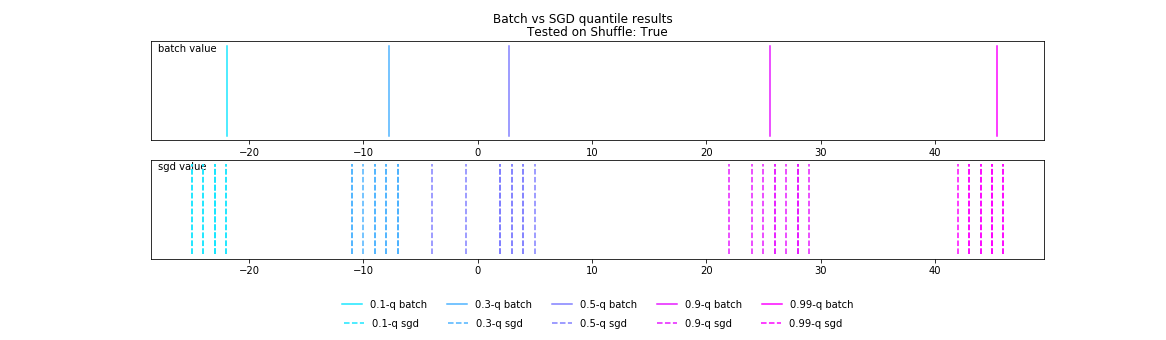
\includegraphics
    [width=1\columnwidth]
    {data_sequence/True_res.png} % Example image
	\caption{
		SGD Estimate Result from Shuffled Data Stream
	}
\end{figure}

\begin{figure}[H] % [h] forces the figure to be output where it is defined in the code (it suppresses floating)
	\centering
    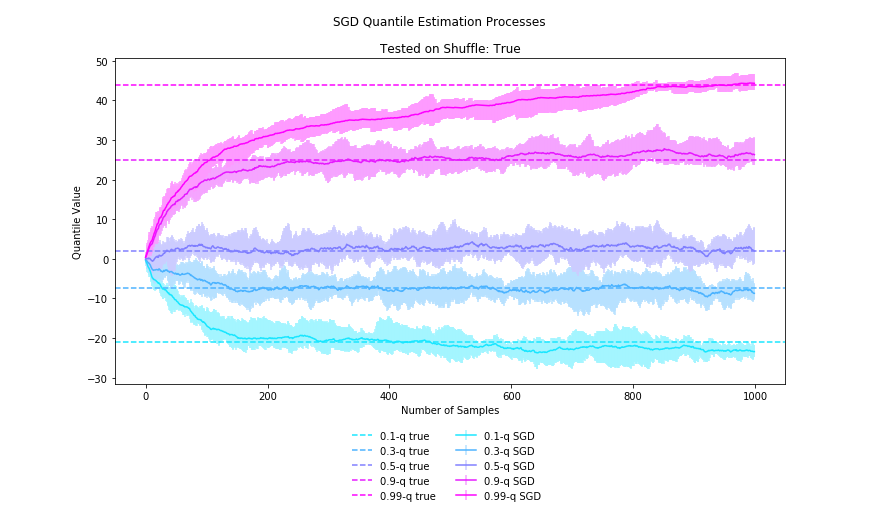
\includegraphics
    [width=1\columnwidth]
    {data_sequence/True_proc.png} % Example image
	\caption{
		SGD Estimate Process from Shuffled Data Stream
	}
\end{figure}

\begin{figure}[H] % [h] forces the figure to be output where it is defined in the code (it suppresses floating)
	\centering
    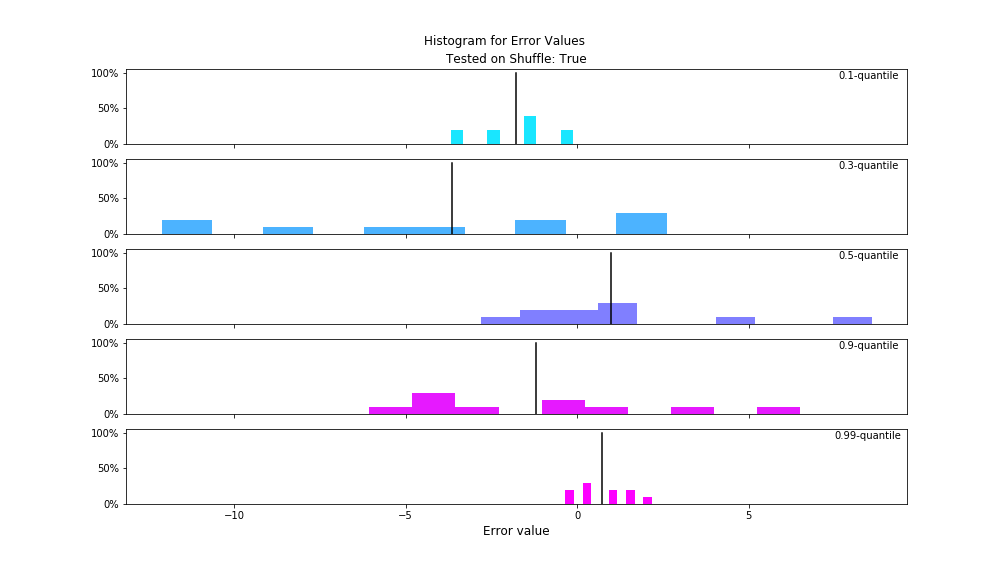
\includegraphics
    [width=1\columnwidth]
    {data_sequence/True_err.png} % Example image
	\caption{
		SGD Estimate Error from Shuffled Data Stream
	}
\end{figure}

\section{Discussion}
\subsection{Failure on Newton's Method}
Newton's method is an iterative method to find the stationary points (where the function's derivative is zero) of a twice-differentiable function $f$. The application of Newton's method failed for our SGD quantile methods, since the loss function of the quantile estimation function is not twice-differentiable. For a specific $\tau$, and $t := x - q$ be the difference between the input data value $x$ and the estimate of quantile $q$, the loss function 
$$
l_\tau(t)= 
    \begin{cases}
        \tau t & t > 0\\
        -(1-\tau) t & otherwise
    \end{cases}
$$
is a linear function of $t$, which doesn't have any second derivative. 
\\\\
Though the method cannot be applied, it is easy to reach the goal of Newton's method: to find the critical points of a function. Instead of stationary point, the loss function has a critical point where it is not differentiable and the derivative changes sign. For any $\tau \in (0,1)$, when $t=0$, the loss function reaches it's critical points at $l_\tau(0) = 0$. Taking the critical point for every step, however, does not contribute to any improvement in quantile estimation. To be at a critical point, the quantile estimate is set to have the equal value of input data $x$, and only in this way we could have $t = x-q = x-x = 0$. Regardless of $\tau$, the quantile estimate is always equal to the value of the latest data point. So far this method has totally failed its goal to estimate a quantile value based on $\tau$ and the entire data stream.
\\\\
From another perspective, the failure of Newton's method is the result of applying large step size for the last input data for a SGD method. In this way, the minimal of current loss function $l_\tau(t)$ is reached, while the total loss function for the input data stream $X$
$$
L_{\tau}(t) = \sum_{x \in X} l_{\tau}(t)
$$
is entirely ignored.
\section{Conclusion}

\end{document}
\end(documentclass)